\documentclass[notes]{subfiles}

\begin{document}
	\addcontentsline{toc}{section}{1.6 - Calculating Limits Using Limit Laws}
	\refstepcounter{section}
	\fancyhead[RO,LE]{\bfseries \large\nameref{cs16}} 
	\fancyhead[LO,RE]{\bfseries \currentname}
	\fancyfoot[C]{{}}
	\fancyfoot[RO,LE]{\large \thepage}	%Footer on Right \thepage is pagenumber
	\fancyfoot[LO,RE]{\large Chapter 1.6}

\section*{Calculating Limits Using Limit Laws}\label{cs16}
	\subsection*{Before Class}
	\addcontentsline{toc}{subsection}{Before Class}
	\subsubsection*{Limit Laws}
	\addcontentsline{toc}{subsubsection}{Limit Laws}
		Since we do not have calculators available to us, we need some tools in order compute limits.  These are given to us a \emph{limit laws}$-$these should be memorized.
		
		\begin{thm}[Limit Laws]
			Suppose that $c$ is a constant, and that the limits $\ds \lim_{x\to a} f(x)$ and $\ds \lim_{x\to a} g(x)$ exist.  Then
			\showto{ins}{
				\begin{enumerate}
					\setlength\itemsep{10pt}
					\item $\ds \lim_{x\to a} [f(x) \pm g(x)] = \ds \lim_{x\to a} f(x) \pm \lim_{x\to a} g(x)$\newline
					\item $\ds \lim_{x\to a} [cf(x)] = c\cdot \lim_{x\to a} f(x)$\newline
					\item $\ds \lim_{x\to a} [f(x)\cdot g(x)] = \lim_{x\to a} f(x)\cdot \lim_{x\to a} g(x)$\newline
					\item $\ds \lim_{x\to a} \dfrac{f(x)}{g(x)} = \dfrac{\ds \lim_{x\to a} f(x)}{\ds \lim_{x\to a} g(x)}$, provided that $\ds \lim_{x\to a} g(x)\neq 0$\newline
					\item $\ds \lim_{x\to a} [f(x)]^n = \left[\lim_{x\to a} f(x)\right]^n$, where $n$ is a positive integer\newline
					\item $\ds \lim_{x\to a} c = c$\newline
					\item $\ds \lim_{x\to a} [f(x)]^{1/n} = \left[\lim_{x\to a} f(x)\right]^{1/n}$, where $n$ is a positive integer (we assume the limit is positive if $n$ is even)\newline
				\end{enumerate}
			}
			\showto{st}{\\ \\
				\begin{enumerate}
					\setlength\itemsep{25pt}
					\item 
					\item 
					\item 
					\item 
					\item 
					\item 
					\item 
				\end{enumerate}
			}			
		\end{thm}
		Each of these can be restated in words.
		\showto{ins}{
			\begin{enumerate}
				\item \textbf{Sum/Difference Rule}: The limit of a sum/difference of functions is the sum/difference of the limit of the functions.
				\item \textbf{Constant Multiplier Rule}: The limit of a constant times a function is the constant times the limit of the function.
				\item \textbf{Product Rule}: The limit of a product of functions is the product of the limits.
				\item \textbf{Quotient Rule}: The limit of a quotient of functions is the quotient of the limits (provided the denominator is nonzero).
				\item \textbf{Power Rule}: The limit of a function raised to a power is the power of the limit of the function.
				\item \textbf{Constant Rule}: The limit of a constant is a constant.
				\item \textbf{Root Rule}: The limit of the $n$th-root of a function is the $n$th-root of the limit of a function.
			\end{enumerate}
		}
		\showto{st}{
			\begin{enumerate}
				\setlength\itemsep{25pt}
				\item 
				\item 
				\item 
				\item 
				\item 
				\item 
				\item 
			\end{enumerate}
		}
		
		\begin{ex}
			Use the limit laws to determine the following limits, if they exist.  The function $f(x)$ is graphed as the solid line, and $g(x)$ is graphed as the dashed line.\\[10pt]
			\begin{minipage}{.38\textwidth}
				\begin{flushleft}
					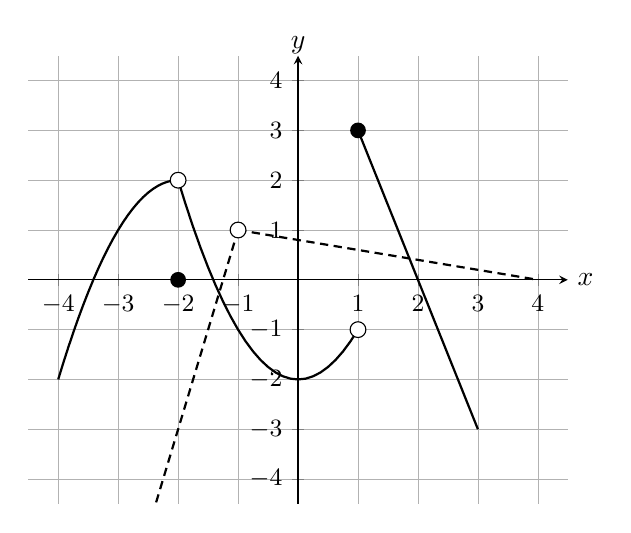
\begin{tikzpicture}
						\begin{axis}[
							grid style = {line width = .1pt, draw = gray!60},
							grid = both,
							every tick label/.append style={font=\small},
							axis x line = middle,
							axis y line = middle,
				    			every axis y label/.style={at={(ticklabel cs:1.15)}, yshift = -3pt},
								y label style={at={(axis description cs: 0.5, 1)},above},
							ytick = {-4,-3,-2,-1,1,2,3,4},
				    			ylabel = {$y$},
				    			ymin = -4.5, ymax = 4.5,
			    				every axis x label/.style= {at ={(ticklabel cs:1)}},
			    				xtick = {-4,-3,-2,-1,1,2,3,4},
				    				x label style={at={(axis description cs: 1, 0.5)},right},
			    				xlabel = {$x$},
			    				xmin = -4.5, xmax = 4.5			
						]	
							\addplot[thick, domain = -4:-2] {-(x+2)^2+2};
								\coordinate (circle1) at (-2,2);
								\coordinate (circle4) at (-2,0);
							\addplot[thick, domain = -2:1] {x^2-2};
							\addplot[thick, densely dashed, domain = -2.5:-1] {4*x+5};
								\coordinate (circle2) at (-1,1);
							\addplot[thick, densely dashed, domain = -1:4] {-.2*x+.8};
							\addplot[thick, domain = 1:3] {-3*x+6};
								\coordinate (circle3) at (1,3);
								\coordinate (circle5) at (1,-1);
						\end{axis}
							\fill[white] (circle1) circle (.1);
							\draw (circle1) circle (0.1);
							\fill (circle4) circle (0.1);
							\fill[white] (circle2) circle (0.1);
							\draw (circle2) circle (0.1);
							\fill[white] (circle5) circle (0.1);
							\draw (circle5) circle (0.1);
							\fill (circle3) circle (0.1);
					\end{tikzpicture}
				\end{flushleft}
			\end{minipage} \hspace{15pt}
			\begin{minipage}{.58\textwidth}
				\begin{flushleft}
					\begin{multicols*}{2}
						\begin{enumerate}[(a)]
							\item $\ds \lim_{x\to 1} [f(x)]$
								\vspace{1in}
							\item $\ds \lim_{x\to -1} [g(x)]$
								\vspace{1in}
							\item $\ds \lim_{x\to -2}\left[\dfrac{f(x)}{g(x)}\right]$
								\vspace{1in}
								\columnbreak 
							\item $\ds \lim_{x\to -1}\left[f(x)g(x)\right]$
								\vspace{1in}
							\item $\ds \lim_{x\to -1}\left[-2f(x)+3g(x)\right]$
								\vspace{1.1in}
							\item $\ds \lim_{x\to 2} [3f(x)]$	
								\vspace{1in}
						\end{enumerate}
							\raggedcolumns
					\end{multicols*}
				\end{flushleft}
			\end{minipage}
		\end{ex}
			\vs{2}
		
		\begin{rmk}[Direct Substitution Property]
			If $f$ is a polynomial, rational, or algebraic function with $a$ in the domain of $f$, then 
			\showto{ins}{
				\[\lim_{x\to a} f(x) = f(a)\]
			}
			\showto{st}{
				\\ \\ \\
			}
		\end{rmk}	
			\vs{1}
			\newpage
			
		\begin{ex}
			Calculate the following limits.  Justify each answer with one (or more) of the limit laws.
			\begin{enumerate}[(a)]
				\item $\ds \lim_{x\to -1} 3x^3+5x^2-7$
					\vs{1}
					
				\item $\ds \lim_{x\to 2} \dfrac{x^3+2x^2-1}{5-3x}$
					\vs{1}
					
				\item $\ds \lim_{x\to 1} \dfrac{x-1}{x^2+1}$
					\vs{1}
					
			\end{enumerate}
		\end{ex}
			\newpage
			
		\begin{question}
			Let $k(x) = \dfrac{x+1}{x^2-1}$.
			\begin{enumerate}[(a)]
				\item The Direct Substitution Property \emph{cannot} be applied to the function at $x = -1$.  Why not?
					\vs{1}
					
				\item Modify the function so that you \emph{can} use the Direct Substitution Property.
					\vs{1}
			\end{enumerate}
		\end{question} 
		\newsec
		
	\subsubsection*{Pre-Class Activities}
	\addcontentsline{toc}{subsubsection}{Pre-Class Activities}
		\begin{ex}
			Assume that $\ds \lim_{x\to 3} f(x) = -1$, $\ds \lim_{x\to 3} g(x) = 2$, and $\ds \lim_{x\to 3} h(x) = 0$.  Find the following limits, if they exist.  If they don't, explain why.  Justify each answer with the appropriate limit law(s).
			\begin{enumerate}[(a)]
				\item $\ds \lim_{x\to 3} [f(x) + 5g(x)]$
					\vs{1}
				\item $\ds \lim_{x\to 3} [f(x)]^5$
					\vs{1}
					\newpage
				
				\item $\ds \lim_{x\to 3} \sqrt{g(x)}$
					\vs{1}
					
				\item $\ds \lim_{x\to 3} \dfrac{3f(x)}{g(x)}$
					\vs{1}
					
				\item $\ds \lim_{x\to 3} \dfrac{g(x)}{h(x)}$
					\vs{1}
					
				\item $\ds \lim_{x\to 3} \dfrac{f(x)h(x)}{g(x)}$
					\vs{1}			
			\end{enumerate}
		\end{ex}
			\newsec
	
	\subsection*{In-Class}
	\addcontentsline{toc}{subsection}{In-Class}
		\begin{ex}
			Compute the following limits:
			\begin{enumerate}[(a)]
				\item $\ds \lim_{t\to -5} g(t)$, where $g(t) = \begin{cases}t^2 -1 & t\neq -5\\ \pi+1 & t = -5 \end{cases}$
					\vs{1}
					\newpage
					
				\item $\ds \lim_{h\to 0} \dfrac{f(x+h)-f(x)}{h}$, where $f(x) = x^2+2x-1$
					\vs{1}
					
				\item $\ds \lim_{h\to 0} \dfrac{f(1+h)-f(1)}{h}$, where $f(x) = \sqrt{x}$
					\vs{1}
			\end{enumerate}
		\end{ex}
			\newpage
			
		\begin{ex}
			Show that $\ds \lim_{x\to a} |x-a| = 0$
		\end{ex}		
			\vs{2.5}
			
		\begin{defn}[Greatest Integer Function]
			The \textbf{greatest integer function}, $\llbracket x\rrbracket$, is 
			\showto{ins}{
				\fbox{the largest integer that is less than or equal to $x$}.
			}
			\showto{st}{
				\\ \\ \\
			}
		\end{defn}
			\vs{.25}
			
		\begin{ex}
			Find $\llbracket x\rrbracket$ for the following values of $x$.
			\begin{enumerate}[(a)]
				\item $x = 2$
					\vs{.25}
					
				\item $x = -1$
					\vs{.25}
					
				\item $x = 5.1$
					\vs{.25}
					
				\item $x = \pi$
					\vs{.25}
					
				\item $x = -6.7$
					\vs{.25}
					
			\end{enumerate}
		\end{ex}		
			\newpage
		
		\begin{ex}
			Find the limits.
			\begin{enumerate}[(a)]
				\item $\ds\lim_{x\to 0.5} \llbracket x \rrbracket$
					\vs{1}
					
				\item $\ds\lim_{x\to 2} \llbracket x\rrbracket$
					\vs{1}
					
				\item $\ds \lim_{x\to 3} \dfrac{\frac{1}{x}-\frac{1}{3}}{x-3}$
					\vs{1}
					
				\item $\ds\lim_{h\to 1} \dfrac{h^4-1}{h^3-1}$
					\vs{1}
					
			\end{enumerate}
		\end{ex}	
			\newpage
			
	\subsubsection*{Two Theorems}
	\addcontentsline{toc}{subsubsection}{Two Theorems}
		\begin{thm}[Limit Inequality]
			If $f(x)\leq g(x)$ when $x$ is near $a$ (except possibly at $a$) and the limits of $f$ and $g$ both exist as $x$ approaches $a$, then
			\showto{ins}{
				\[\lim_{x\to a} f(x)\leq \lim_{x\to a} g(x)\]
			}
			\showto{st}{
				\\ \\ \\
			}
		\end{thm}
			
		
		\begin{thm}[Squeeze Theorem]
			If $f(x)\leq g(x)\leq h(x)$ when $x$ is near $a$ (except possibly at $a$) and
			\showto{ins}{
				\[\lim_{x\to a} f(x) = \lim_{x\to a} h(x) = L\]
				then
				\[\lim_{x\to a} g(x) = L\]
			}
			\showto{st}{
				\\ \\ \\ \\ \\ \\
			}
		\end{thm}
		
		\begin{ex}
			Use the Squeeze Theorem to show that $\ds \lim_{x\to 0} x^2 \sin \lrpar{\dfrac{1}{x}}= 0$
		\end{ex}
			\newpage
			
	\subsection*{After Class}
	\addcontentsline{toc}{subsection}{After Class}
		\begin{ex}
			If $2x\leq g(x) \leq x^6 - x^4 + 2$ for all $x$, find $\ds \lim_{x\to 1} g(x)$.
		\end{ex}
			\vs{1}
			
		\begin{ex}
			The \emph{signum function} (or the \emph{sign function}), $\text{sgn}(x)$, is given by \[\text{sgn}(x) = \begin{cases}-1 & x < 0\\ 0 & x = 0\\ 1 & x > 0 \end{cases}\]  
			\begin{enumerate}[(a)]
				\item Sketch the graph of $\text{sgn}(x)$.
					\vs{1}
					
				\item Find the limits, or explain why they don't exist:
					\begin{enumerate}[(a)]
						\item $\ds \lim_{x\to 0} \text{sgn}(x)$
							\vs{.5}
						\item $\ds \lim_{x\to 0} |\text{sgn}(x)|$
							\vs{.5}
					\end{enumerate}
			\end{enumerate}
		\end{ex}

		
			\newpage
			
		\begin{ex}
			Find the limit: 
			\begin{enumerate}[(a)]
				\item $\ds \lim_{x\to -4} \dfrac{3x + 12}{|x + 4|}$
					\vs{1}
				\item $\ds \lim_{x\to 2} \dfrac{\sqrt{4x+1} - 3}{x-2}$
					\vs{1}
				\item $\ds \lim_{x\to -1} \dfrac{2x^2 + 3x + 1}{x^2 - 2x -3}$
					\vs{1}
				\item $\ds \lim_{h\to 0} \dfrac{(x+h)^3 - x^3}{h}$
					\vs{1}
			\end{enumerate}
		\end{ex}
	\clearpage
\end{document}